\section{Аналитическая часть}

\subsection{Постановка задачи}\label{sec:task}
По заданию требуется разработать драйвер в виде загружаемого модуля ядра, позволяющий управлять устройствами, подключенными с помощью интерфейса GPIO.

Необходимо предоставить пользователю возможность ввода/вывода информации с устройств, управления режимами.

Для достижения данной цели необходимо решить следующие задачи:
\begin{enumerate}
	\item ознакомиться с основными принципами работы устройств интерфейса GPIO;
	\item определить способ управления устройствами;
	\item выделить набор действий;
	\item реализовать драйвер.
\end{enumerate}

\subsection{Принцип работы устройств GPIO}
\textbf{GPIO} - интерфейс для связи между компонентами компьютерной системы, к примеру, микропроцессором и различными периферийными устройствами\cite{subj:def}. Контакты GPIO могут выступать как в роли входа, так и в роли выхода — это, как правило, конфигурируется. Обычно они используются для подключения датчиков, переключателей, дисплеев и т.п.

В данной работе будет использоваться одноплатный компьютер Raspberry Pi 2B ввиду отсутствия в распоряжении других компьютеров. Рассмотрим подробнее организацию GPIO на его примере.

На рисунке \ref{pic:gpio} описывается назначение каждого из контактов (пинов)  для этой модели. Можно отметить, что не все из них используются для ввода/вывода. Помимо этого есть контакты предназначенные для подачи определённого напряжения на внешние устройства (3.3V, 5V) или для заземления (GROUND).

\begin{figure}[h!] 
	\begin{center}
		{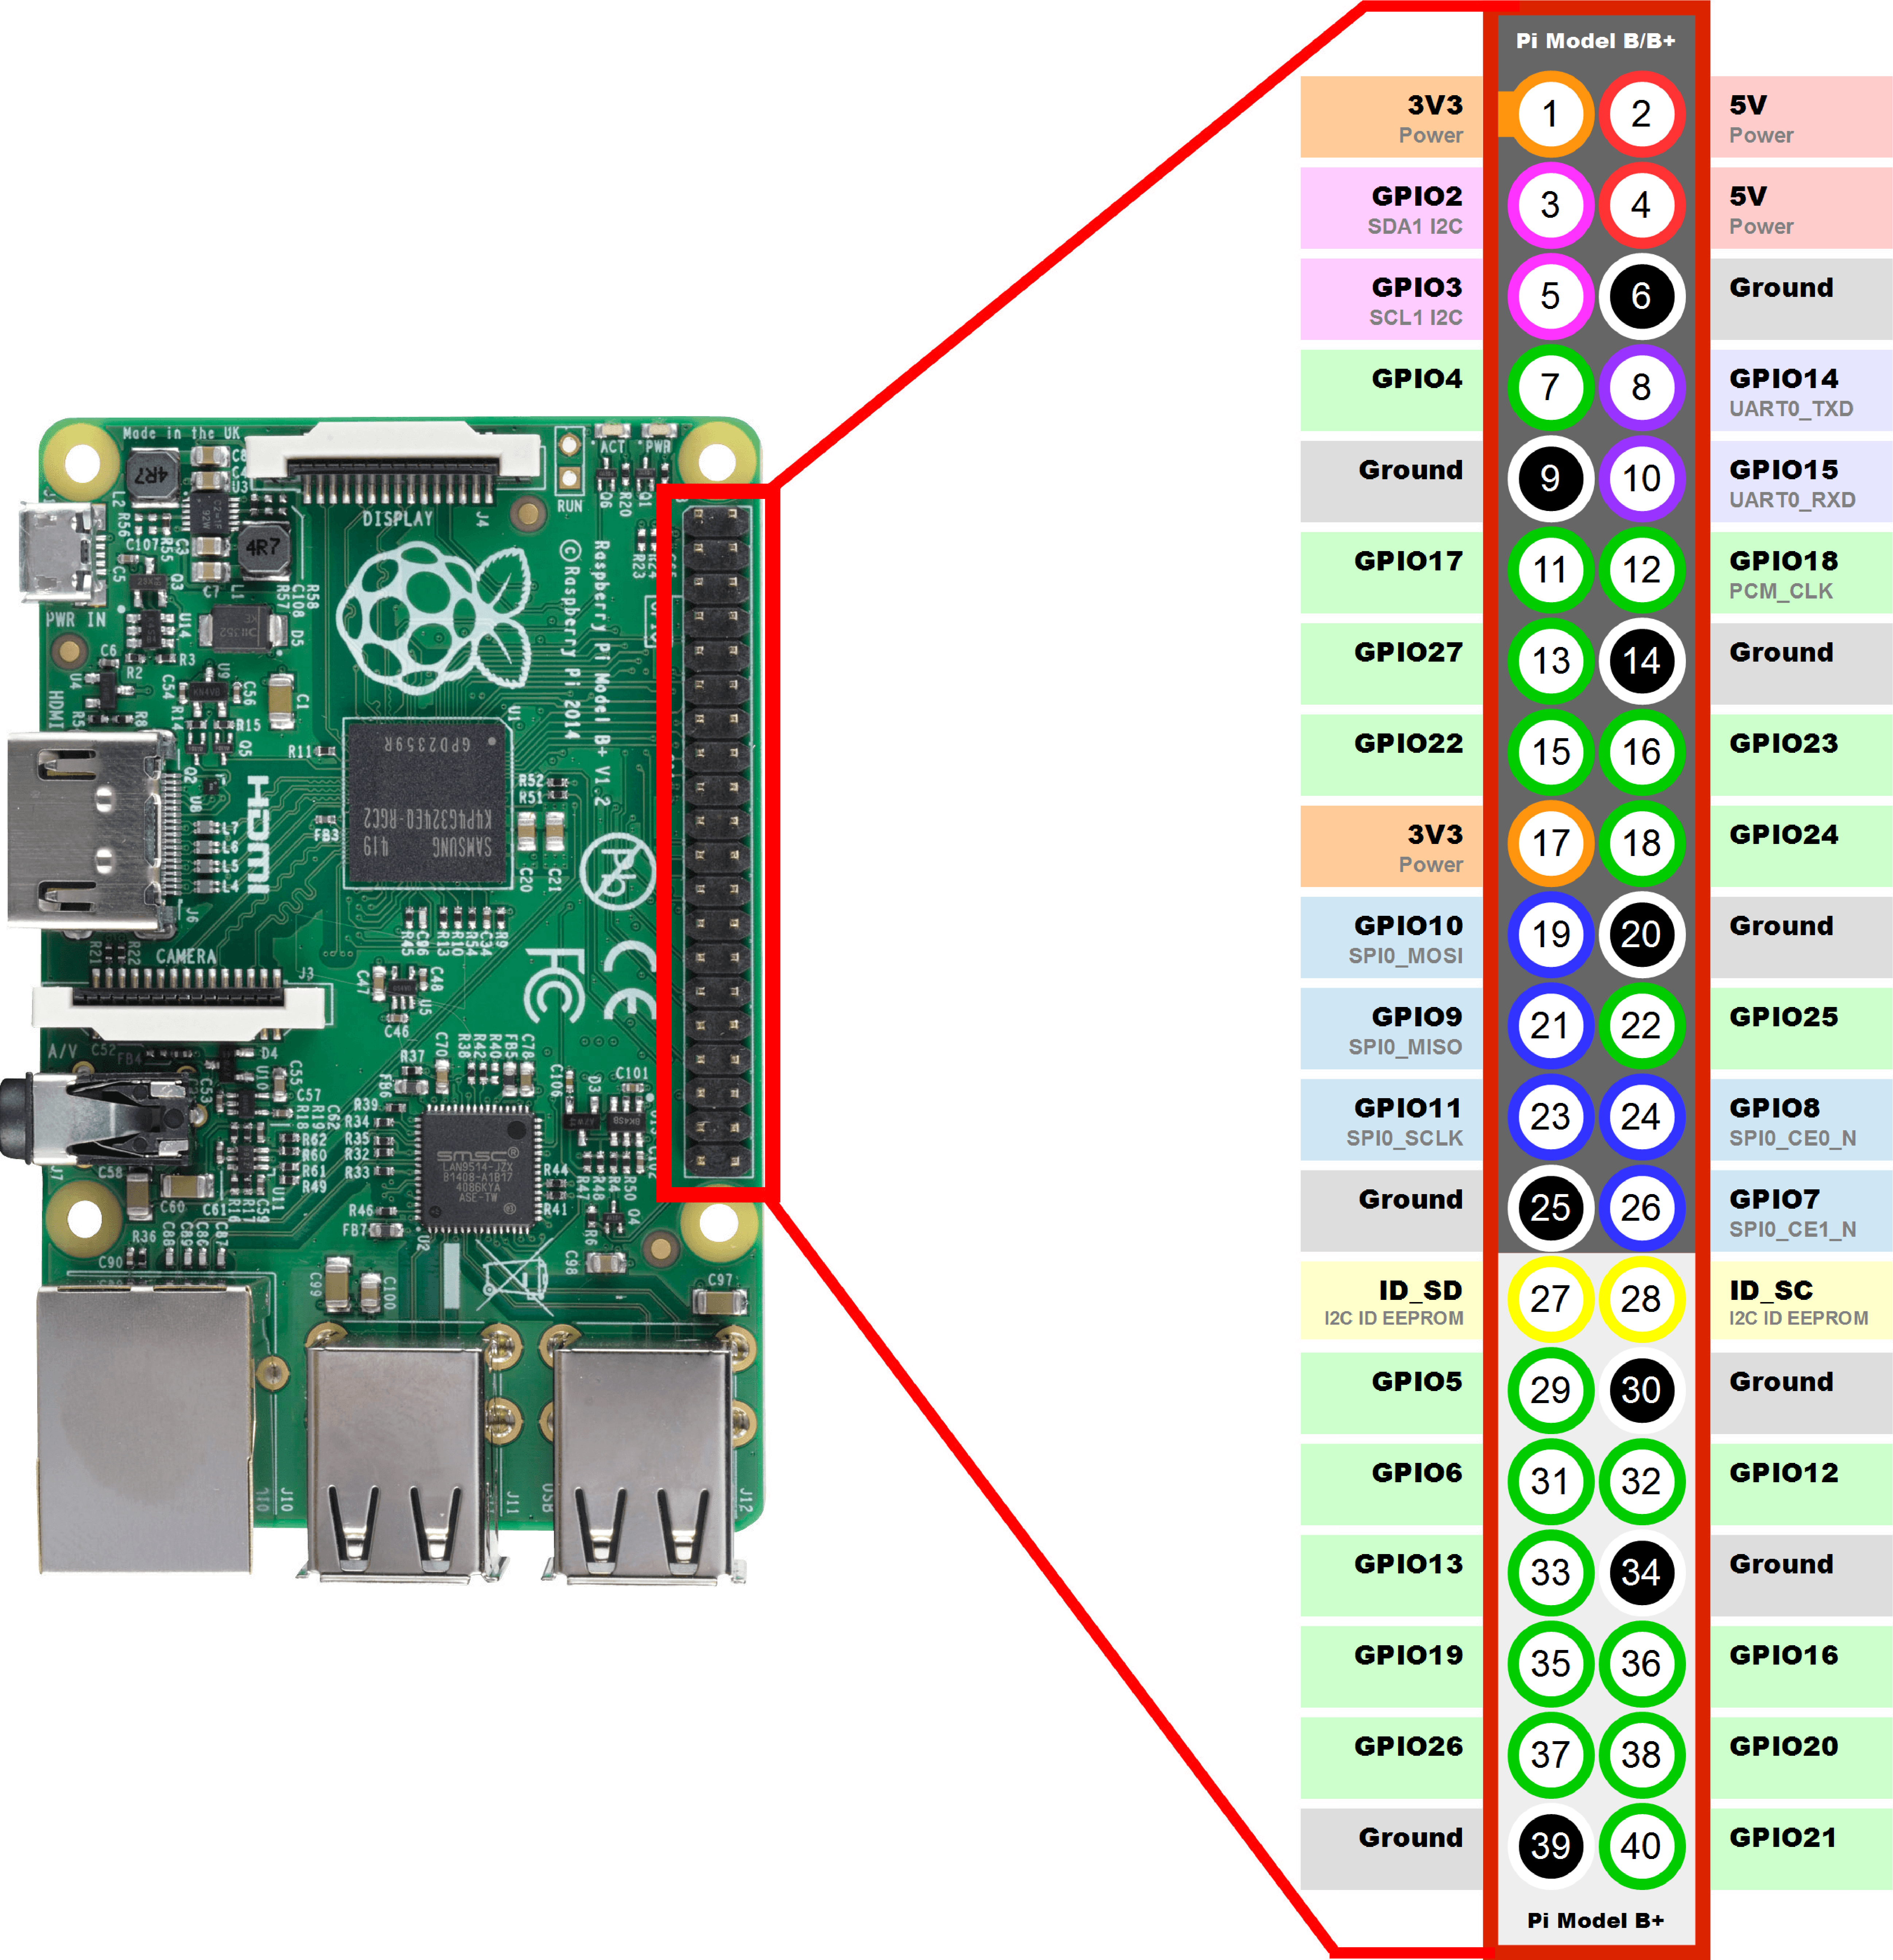
\includegraphics[scale=0.15, angle=0]{img/gpio.pdf}}
		\caption{Назначение пинов Raspberry Pi 2B}
		\label{pic:gpio}
	\end{center}
\end{figure}

Пин GPIO имеет два режима:
\begin{itemize}
	\item \textbf{Вход}. Напряжение подаётся внешним устройством. От +0.0В до +1.8В считается уровнем логического нуля, +1.8В-3.3В - логическая единица.
	\item \textbf{Выход}. Напряжение подаётся самим Raspberry Pi. Уровень логических 0 и 1 аналогичный.
\end{itemize}

По сути, передача и приём информации осуществляется только считыванием и установлением определённого напряжения. Выходы, отмеченные на схеме зелёным цветом имеют наиболее простой принцип действия: режим ввода/вывода в них устанавливается на всё время подключения устройства, а значение напряжения является относительно постоянным, так как по ним передаётся минимальное количество информации. 

В отличие от них, контакты имеющие подпись I2C, SPI или UART используются для последовательный синхронной передачи данных в режиме полного или полудуплекса. Это означает, что они используются для передачи уже более большого количества данных и могут переключать режим ввода/вывода по несколько тысяч раз за секунду. 

Целью данной работы является разработка базового взаимодействия с внешними устройствами, поэтому  драйвер будет ориентирован на более простые интерфейсы GPIO.


\subsection{Способ управления}
Следующей задачей является определение способа чтения и изменения состояния интерфейсов GPIO.

Для работы с пинами используется способ отображения в память (memory maping). Для чтения или изменения состояния устройства требуется взаимодействовать с определённым участком оперативной память, имеющей постоянный физический адрес. Для выполнения подобных действий требуется иметь нулевой уровень привелегий, поэтому программа должна быть реализована в виде загружаемого модуля ядра.

Рассмотрим устройство отображения GPIO в память для Raspberry Pi 2B. В листинге \ref{lst:mapping_const} приведены используемые константы.
\begin{lstlisting}[caption = {struct module}, label=lst:mapping_const]
#define BCM2708_PERI_BASE	0x3F000000
#define GPIO_BASE           (BCM2708_PERI_BASE + 0x200000) 	

/* GPIO register offsets */
#define GPFSEL0		0x0		/* Function Select */
#define GPSET0		0x1c	/* Pin Output Set */
#define GPCLR0		0x28	/* Pin Output Clear */
#define GPLEV0		0x34	/* Pin Level */
...
\end{lstlisting}

Адрес \textbf{BCM2708_PERI_BASE} определяет начало участка memory mapping для периферийных устройств, участок GPIO имеет смещение $0x200000$. Далее представленны смещения участков памяти относительно базового адреса \textbf{GPIO_BASE}, каждое из которых отвечает соответственно за режим ввода/вывода, установку значения, сброс значения и чтение значения с пинов.

\subsection{Выводы}
В этом разделе были сформулированы цель и задачи, рассмотрены основные этапы, также подробно изучены принципы работы межсетевого экрана. 

Для достижения поставленной цели было принято решение использовать простой misc драйвер, поскольку он ориентирован на выполнение небольших задач и имеет упрощённую схему создания.


